\documentclass[]{article}
\usepackage{lmodern}
\usepackage{amssymb,amsmath}
\usepackage{ifxetex,ifluatex}
\usepackage{fixltx2e} % provides \textsubscript
\ifnum 0\ifxetex 1\fi\ifluatex 1\fi=0 % if pdftex
  \usepackage[T1]{fontenc}
  \usepackage[utf8]{inputenc}
\else % if luatex or xelatex
  \ifxetex
    \usepackage{mathspec}
  \else
    \usepackage{fontspec}
  \fi
  \defaultfontfeatures{Ligatures=TeX,Scale=MatchLowercase}
\fi
% use upquote if available, for straight quotes in verbatim environments
\IfFileExists{upquote.sty}{\usepackage{upquote}}{}
% use microtype if available
\IfFileExists{microtype.sty}{%
\usepackage{microtype}
\UseMicrotypeSet[protrusion]{basicmath} % disable protrusion for tt fonts
}{}
\usepackage[margin=1in]{geometry}
\usepackage{hyperref}
\hypersetup{unicode=true,
            pdftitle={Normal\_cor\_simulation},
            pdfauthor={Xuelong Wang},
            pdfborder={0 0 0},
            breaklinks=true}
\urlstyle{same}  % don't use monospace font for urls
\usepackage{graphicx,grffile}
\makeatletter
\def\maxwidth{\ifdim\Gin@nat@width>\linewidth\linewidth\else\Gin@nat@width\fi}
\def\maxheight{\ifdim\Gin@nat@height>\textheight\textheight\else\Gin@nat@height\fi}
\makeatother
% Scale images if necessary, so that they will not overflow the page
% margins by default, and it is still possible to overwrite the defaults
% using explicit options in \includegraphics[width, height, ...]{}
\setkeys{Gin}{width=\maxwidth,height=\maxheight,keepaspectratio}
\IfFileExists{parskip.sty}{%
\usepackage{parskip}
}{% else
\setlength{\parindent}{0pt}
\setlength{\parskip}{6pt plus 2pt minus 1pt}
}
\setlength{\emergencystretch}{3em}  % prevent overfull lines
\providecommand{\tightlist}{%
  \setlength{\itemsep}{0pt}\setlength{\parskip}{0pt}}
\setcounter{secnumdepth}{5}
% Redefines (sub)paragraphs to behave more like sections
\ifx\paragraph\undefined\else
\let\oldparagraph\paragraph
\renewcommand{\paragraph}[1]{\oldparagraph{#1}\mbox{}}
\fi
\ifx\subparagraph\undefined\else
\let\oldsubparagraph\subparagraph
\renewcommand{\subparagraph}[1]{\oldsubparagraph{#1}\mbox{}}
\fi

%%% Use protect on footnotes to avoid problems with footnotes in titles
\let\rmarkdownfootnote\footnote%
\def\footnote{\protect\rmarkdownfootnote}

%%% Change title format to be more compact
\usepackage{titling}

% Create subtitle command for use in maketitle
\newcommand{\subtitle}[1]{
  \posttitle{
    \begin{center}\large#1\end{center}
    }
}

\setlength{\droptitle}{-2em}

  \title{Normal\_cor\_simulation}
    \pretitle{\vspace{\droptitle}\centering\huge}
  \posttitle{\par}
    \author{Xuelong Wang}
    \preauthor{\centering\large\emph}
  \postauthor{\par}
      \predate{\centering\large\emph}
  \postdate{\par}
    \date{2018-07-25}

\usepackage{booktabs}
\usepackage{longtable}
\usepackage{array}
\usepackage{multirow}
\usepackage[table]{xcolor}
\usepackage{wrapfig}
\usepackage{float}
\usepackage{colortbl}
\usepackage{pdflscape}
\usepackage{tabu}
\usepackage{threeparttable}
\usepackage{threeparttablex}
\usepackage[normalem]{ulem}
\usepackage{makecell}

\usepackage{float,amsmath, bbm, siunitx, bm}
\floatplacement{figure}{H}
\newcommand{\indep}{\rotatebox[origin=c]{90}{$\models$}}

\begin{document}
\maketitle

{
\setcounter{tocdepth}{2}
\tableofcontents
}
\section{Motivation}\label{motivation}

\section{Simulation result}\label{simulation-result}

\subsection{Setup}\label{setup}

\subsubsection{Averaged estimation}\label{averaged-estimation}

\rowcolors{2}{gray!80}{white}

\begin{table}[!h]

\caption{\label{tab:full data norm}correlation-0.1-null}
\centering
\begin{tabular}[t]{r|r|r|r|r|r}
\hiderowcolors
\hline
\multicolumn{3}{c|}{Main} & \multicolumn{3}{|c}{Interaction} \\
\cline{1-3} \cline{4-6}
true\_main & GCTA\_main & prop\_main & true\_interaction & GCTA\_interaction & prop\_interaction\\
\hline
\showrowcolors
3.088373 & 2.2629134 & 2.6810971 & 6.445714 & 7.7078883 & 6.3421346\\
\hline
0.000000 & 0.5095913 & 0.4890747 & 0.000000 & 1.4190317 & 0.9831575\\
\hline
3.712037 & 3.2604039 & 4.0312605 & 4.752567 & 5.3313724 & 5.6001181\\
\hline
0.000000 & 0.5476864 & 0.5132892 & 0.000000 & 1.0871311 & 1.0439581\\
\hline
2.681057 & 2.1712492 & 2.9792021 & 5.469751 & 3.6457060 & 6.1875434\\
\hline
0.000000 & 0.3667526 & 0.4521873 & 0.000000 & 0.7242043 & 0.9909888\\
\hline
\end{tabular}
\end{table}

\rowcolors{2}{white}{white} \rowcolors{2}{gray!80}{white}

\begin{table}[!h]

\caption{\label{tab:full data norm}correlation-0.2-null}
\centering
\begin{tabular}[t]{r|r|r|r|r|r}
\hiderowcolors
\hline
\multicolumn{3}{c|}{Main} & \multicolumn{3}{|c}{Interaction} \\
\cline{1-3} \cline{4-6}
true\_main & GCTA\_main & prop\_main & true\_interaction & GCTA\_interaction & prop\_interaction\\
\hline
\showrowcolors
3.053130 & 2.2170802 & 2.6678900 & 6.214107 & 6.4985646 & 5.6397438\\
\hline
0.000000 & 0.5944800 & 0.4480933 & 0.000000 & 1.4905036 & 1.0466755\\
\hline
3.553199 & 1.8826877 & 3.4683129 & 4.475504 & 1.1963946 & 4.0876341\\
\hline
0.000000 & 0.4518005 & 0.5279246 & 0.000000 & 0.3304510 & 0.8316342\\
\hline
2.346156 & 0.9602659 & 2.4056761 & 5.452543 & 1.5006302 & 5.3123168\\
\hline
0.000000 & 0.2237377 & 0.4383947 & 0.000000 & 0.2875944 & 0.8173162\\
\hline
\end{tabular}
\end{table}

\rowcolors{2}{white}{white} \rowcolors{2}{gray!80}{white}

\begin{table}[!h]

\caption{\label{tab:full data norm}correlation-0.3-null}
\centering
\begin{tabular}[t]{r|r|r|r|r|r}
\hiderowcolors
\hline
\multicolumn{3}{c|}{Main} & \multicolumn{3}{|c}{Interaction} \\
\cline{1-3} \cline{4-6}
true\_main & GCTA\_main & prop\_main & true\_interaction & GCTA\_interaction & prop\_interaction\\
\hline
\showrowcolors
2.923335 & 3.1116123 & 3.0790003 & 7.493621 & 9.9872651 & 6.7525273\\
\hline
0.000000 & 0.7168690 & 0.4625207 & 0.000000 & 1.5570798 & 1.1331375\\
\hline
3.177118 & 1.4836731 & 2.9450186 & 4.135163 & 0.5568038 & 3.6233722\\
\hline
0.000000 & 0.5075044 & 0.4244663 & 0.000000 & 0.2191097 & 0.7248550\\
\hline
2.082130 & 0.6638717 & 1.8373159 & 4.419051 & 0.8571361 & 3.5220102\\
\hline
0.000000 & 0.2459053 & 0.3655716 & 0.000000 & 0.3173453 & 0.7818311\\
\hline
\end{tabular}
\end{table}

\rowcolors{2}{white}{white} \rowcolors{2}{gray!80}{white}

\begin{table}[!h]

\caption{\label{tab:full data norm}correlation-0.4-null}
\centering
\begin{tabular}[t]{r|r|r|r|r|r}
\hiderowcolors
\hline
\multicolumn{3}{c|}{Main} & \multicolumn{3}{|c}{Interaction} \\
\cline{1-3} \cline{4-6}
true\_main & GCTA\_main & prop\_main & true\_interaction & GCTA\_interaction & prop\_interaction\\
\hline
\showrowcolors
2.967121 & 3.1046591 & 3.6375580 & 8.101689 & 10.4165112 & 6.5820007\\
\hline
0.000000 & 0.7063818 & 0.5403943 & 0.000000 & 1.5469132 & 0.9358535\\
\hline
2.900933 & 1.2218489 & 2.9546162 & 3.773409 & 0.2746577 & 3.3916797\\
\hline
0.000000 & 0.4011364 & 0.4510457 & 0.000000 & 0.0878513 & 0.7950213\\
\hline
1.843065 & 0.4277090 & 1.9797686 & 3.880287 & 0.2210265 & 3.1506855\\
\hline
0.000000 & 0.1895094 & 0.3919166 & 0.000000 & 0.0959511 & 0.6900077\\
\hline
\end{tabular}
\end{table}

\rowcolors{2}{white}{white} \rowcolors{2}{gray!80}{white}

\begin{table}[!h]

\caption{\label{tab:full data norm}correlation-0.5-null}
\centering
\begin{tabular}[t]{r|r|r|r|r|r}
\hiderowcolors
\hline
\multicolumn{3}{c|}{Main} & \multicolumn{3}{|c}{Interaction} \\
\cline{1-3} \cline{4-6}
true\_main & GCTA\_main & prop\_main & true\_interaction & GCTA\_interaction & prop\_interaction\\
\hline
\showrowcolors
2.945555 & 2.1497417 & 2.7830068 & 9.512110 & 8.6159597 & 7.4123267\\
\hline
0.000000 & 0.4807449 & 0.4245746 & 0.000000 & 1.1259187 & 1.0134897\\
\hline
2.704770 & 1.7836148 & 2.9072267 & 3.141388 & 0.1504048 & 3.0310716\\
\hline
0.000000 & 0.4878225 & 0.5350919 & 0.000000 & 0.1054500 & 0.8478031\\
\hline
1.684237 & 0.5280842 & 1.5990481 & 3.550564 & 0.1247029 & 2.8454342\\
\hline
0.000000 & 0.2146278 & 0.3474024 & 0.000000 & 0.0435080 & 0.7950938\\
\hline
\end{tabular}
\end{table}

\rowcolors{2}{white}{white} \rowcolors{2}{gray!80}{white}

\begin{table}[!h]

\caption{\label{tab:full data norm}correlation-0.6-null}
\centering
\begin{tabular}[t]{r|r|r|r|r|r}
\hiderowcolors
\hline
\multicolumn{3}{c|}{Main} & \multicolumn{3}{|c}{Interaction} \\
\cline{1-3} \cline{4-6}
true\_main & GCTA\_main & prop\_main & true\_interaction & GCTA\_interaction & prop\_interaction\\
\hline
\showrowcolors
2.840187 & 3.4255557 & 3.6075327 & 13.183739 & 11.3110130 & 12.6503986\\
\hline
0.000000 & 0.6164349 & 0.5497321 & 0.000000 & 0.9272107 & 1.2512915\\
\hline
2.620650 & 1.5387039 & 2.5066288 & 3.032240 & 0.1204276 & 3.0714704\\
\hline
0.000000 & 0.3709169 & 0.3816089 & 0.000000 & 0.0789471 & 0.8263944\\
\hline
1.362578 & 0.5149362 & 1.2847950 & 3.172002 & 0.1199249 & 2.8407743\\
\hline
0.000000 & 0.2235774 & 0.3522378 & 0.000000 & 0.0850224 & 0.6474535\\
\hline
\end{tabular}
\end{table}

\rowcolors{2}{white}{white} \rowcolors{2}{gray!80}{white}

\begin{table}[!h]

\caption{\label{tab:full data norm}correlation-0.7-null}
\centering
\begin{tabular}[t]{r|r|r|r|r|r}
\hiderowcolors
\hline
\multicolumn{3}{c|}{Main} & \multicolumn{3}{|c}{Interaction} \\
\cline{1-3} \cline{4-6}
true\_main & GCTA\_main & prop\_main & true\_interaction & GCTA\_interaction & prop\_interaction\\
\hline
\showrowcolors
2.921671 & 2.3387362 & 2.8414534 & 14.876244 & 11.7346465 & 14.3432345\\
\hline
0.000000 & 0.4934600 & 0.4930917 & 0.000000 & 0.8654897 & 1.1592587\\
\hline
2.202138 & 1.1621946 & 1.9412529 & 2.563225 & 0.0337007 & 2.3039060\\
\hline
0.000000 & 0.3361885 & 0.3905409 & 0.000000 & 0.0318753 & 0.8395119\\
\hline
1.205999 & 0.5551601 & 1.1075252 & 3.059272 & 0.1667304 & 3.0455072\\
\hline
0.000000 & 0.2216231 & 0.3112669 & 0.000000 & 0.0908275 & 0.8467851\\
\hline
\end{tabular}
\end{table}

\rowcolors{2}{white}{white} \rowcolors{2}{gray!80}{white}

\begin{table}[!h]

\caption{\label{tab:full data norm}correlation-0.8-null}
\centering
\begin{tabular}[t]{r|r|r|r|r|r}
\hiderowcolors
\hline
\multicolumn{3}{c|}{Main} & \multicolumn{3}{|c}{Interaction} \\
\cline{1-3} \cline{4-6}
true\_main & GCTA\_main & prop\_main & true\_interaction & GCTA\_interaction & prop\_interaction\\
\hline
\showrowcolors
2.6688253 & 3.5039081 & 3.9745800 & 17.532693 & 11.7821539 & 18.3254286\\
\hline
0.0000000 & 0.5739670 & 0.6092979 & 0.000000 & 0.7556400 & 1.6198094\\
\hline
1.9782238 & 1.5076674 & 2.1516555 & 1.362698 & 0.0071326 & 1.3309489\\
\hline
0.0000000 & 0.3669671 & 0.4215761 & 0.000000 & 0.0231179 & 0.7670574\\
\hline
0.8447751 & 0.3164986 & 0.7481253 & 1.934832 & 0.0885135 & 1.7759901\\
\hline
0.0000000 & 0.1632832 & 0.2611656 & 0.000000 & 0.0668263 & 0.6656269\\
\hline
\end{tabular}
\end{table}

\rowcolors{2}{white}{white} \rowcolors{2}{gray!80}{white}

\begin{table}[!h]

\caption{\label{tab:full data norm}correlation-0.9-null}
\centering
\begin{tabular}[t]{r|r|r|r|r|r}
\hiderowcolors
\hline
\multicolumn{3}{c|}{Main} & \multicolumn{3}{|c}{Interaction} \\
\cline{1-3} \cline{4-6}
true\_main & GCTA\_main & prop\_main & true\_interaction & GCTA\_interaction & prop\_interaction\\
\hline
\showrowcolors
2.6570991 & 1.7946098 & 2.1760449 & 23.6527893 & 12.1641929 & 25.8535477\\
\hline
0.0000000 & 0.3427883 & 0.4199620 & 0.0000000 & 0.6071203 & 1.6459841\\
\hline
1.6713933 & 1.2925165 & 1.4944993 & 0.8595516 & 0.0311803 & 0.8747202\\
\hline
0.0000000 & 0.2978465 & 0.3466506 & 0.0000000 & 0.0332608 & 0.6366171\\
\hline
0.6484439 & 0.4155443 & 0.6954721 & 1.1294039 & 0.1208959 & 1.0610190\\
\hline
0.0000000 & 0.1935329 & 0.2713971 & 0.0000000 & 0.0702455 & 0.6781311\\
\hline
\end{tabular}
\end{table}

\rowcolors{2}{white}{white}

\clearpage

\subsubsection{Histgram of 100
iterations}\label{histgram-of-100-iterations}

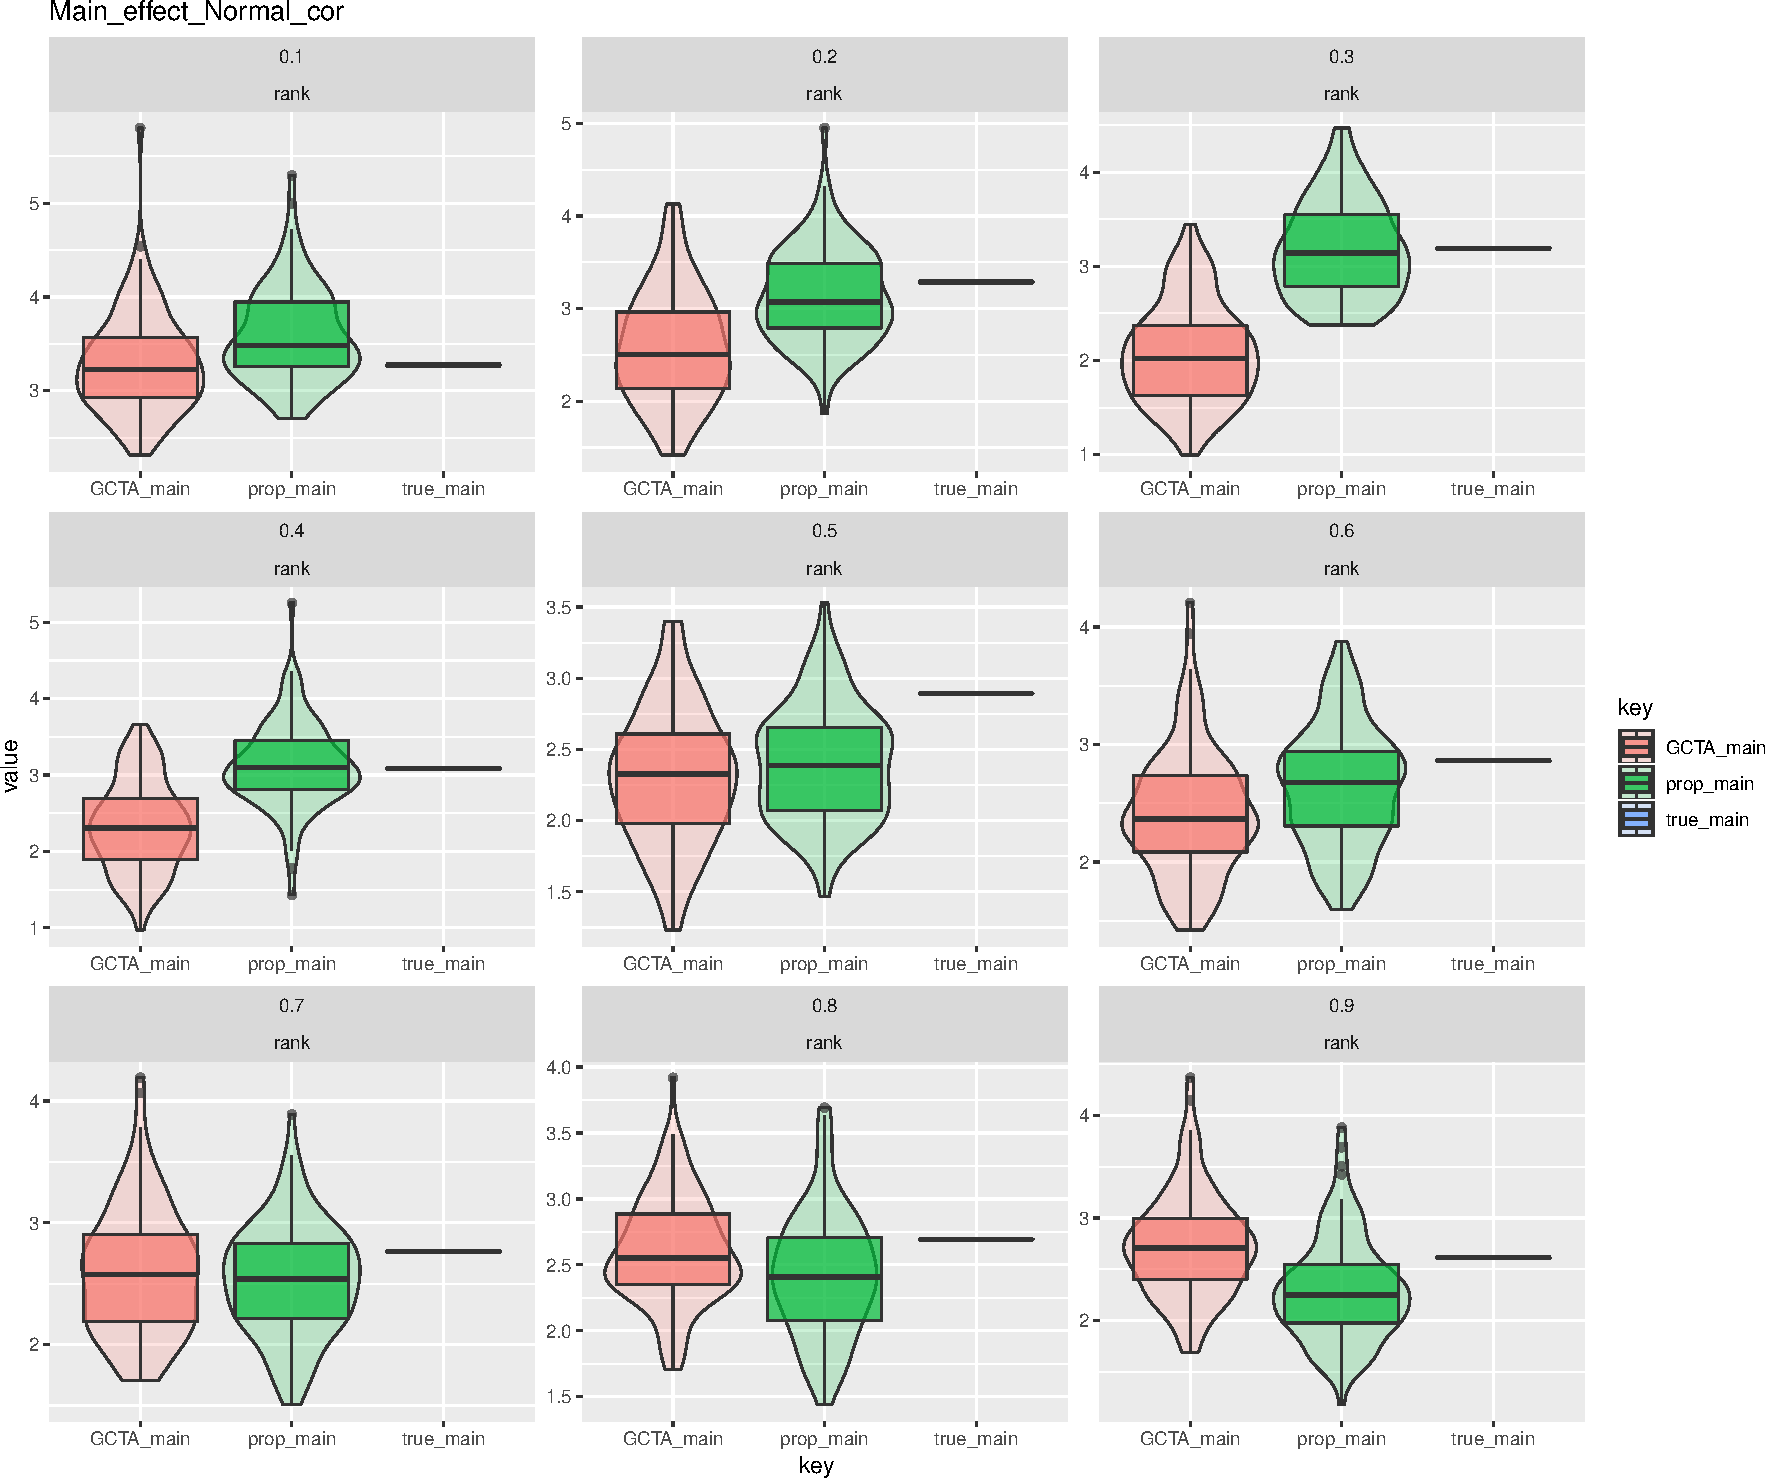
\includegraphics{Norl_cor_simulation_files/figure-latex/normal_main-1.pdf}

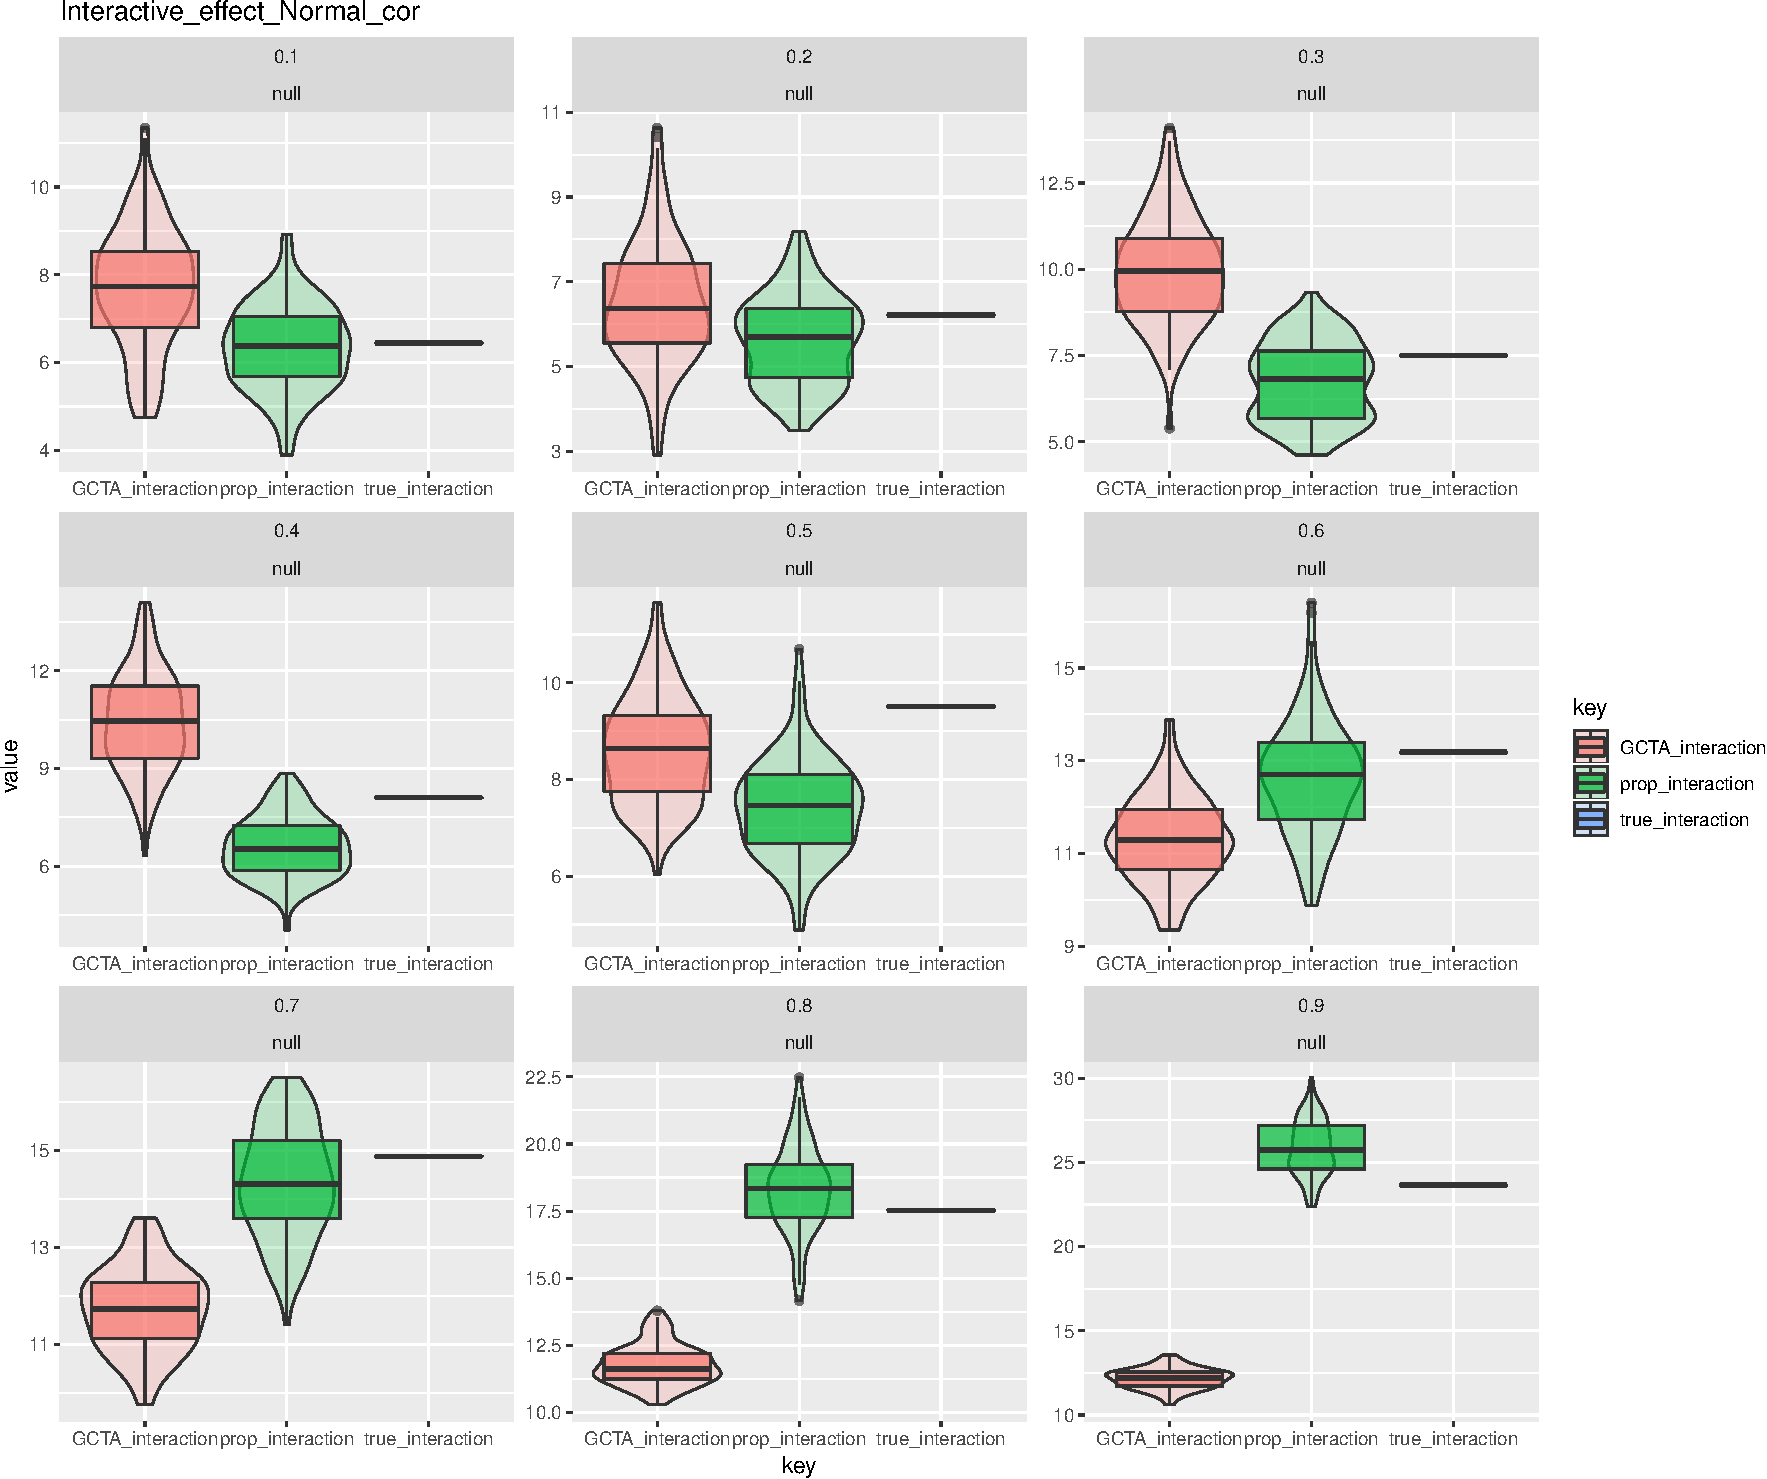
\includegraphics{Norl_cor_simulation_files/figure-latex/normal_inter-1.pdf}

\subsubsection{Averaged estimation}\label{averaged-estimation-1}

\rowcolors{2}{gray!80}{white}

\begin{table}[!h]

\caption{\label{tab:full data chi}-null}
\centering
\begin{tabular}[t]{r|r|r|r|r|r}
\hiderowcolors
\hline
\multicolumn{3}{c|}{Main} & \multicolumn{3}{|c}{Interaction} \\
\cline{1-3} \cline{4-6}
true\_main & GCTA\_main & prop\_main & true\_interaction & GCTA\_interaction & prop\_interaction\\
\hline
\showrowcolors
3.206260 & 2.4278846 & 2.3987387 & 6.053616 & 2.7948026 & 3.2127886\\
\hline
0.000000 & 0.4877009 & 0.4836191 & 0.000000 & 0.6241777 & 0.6946283\\
\hline
4.184742 & 3.7079258 & 3.6457226 & 5.662183 & 5.0952825 & 5.4150564\\
\hline
0.000000 & 0.6460932 & 0.6383936 & 0.000000 & 1.0122512 & 1.0203281\\
\hline
2.751369 & 2.0729482 & 2.2093535 & 5.967688 & 3.0214403 & 2.9723835\\
\hline
0.000000 & 0.4635415 & 0.4757792 & 0.000000 & 0.6891246 & 0.7034145\\
\hline
\end{tabular}
\end{table}

\rowcolors{2}{white}{white}

\clearpage

\subsubsection{Histgram of 100
iterations}\label{histgram-of-100-iterations-1}

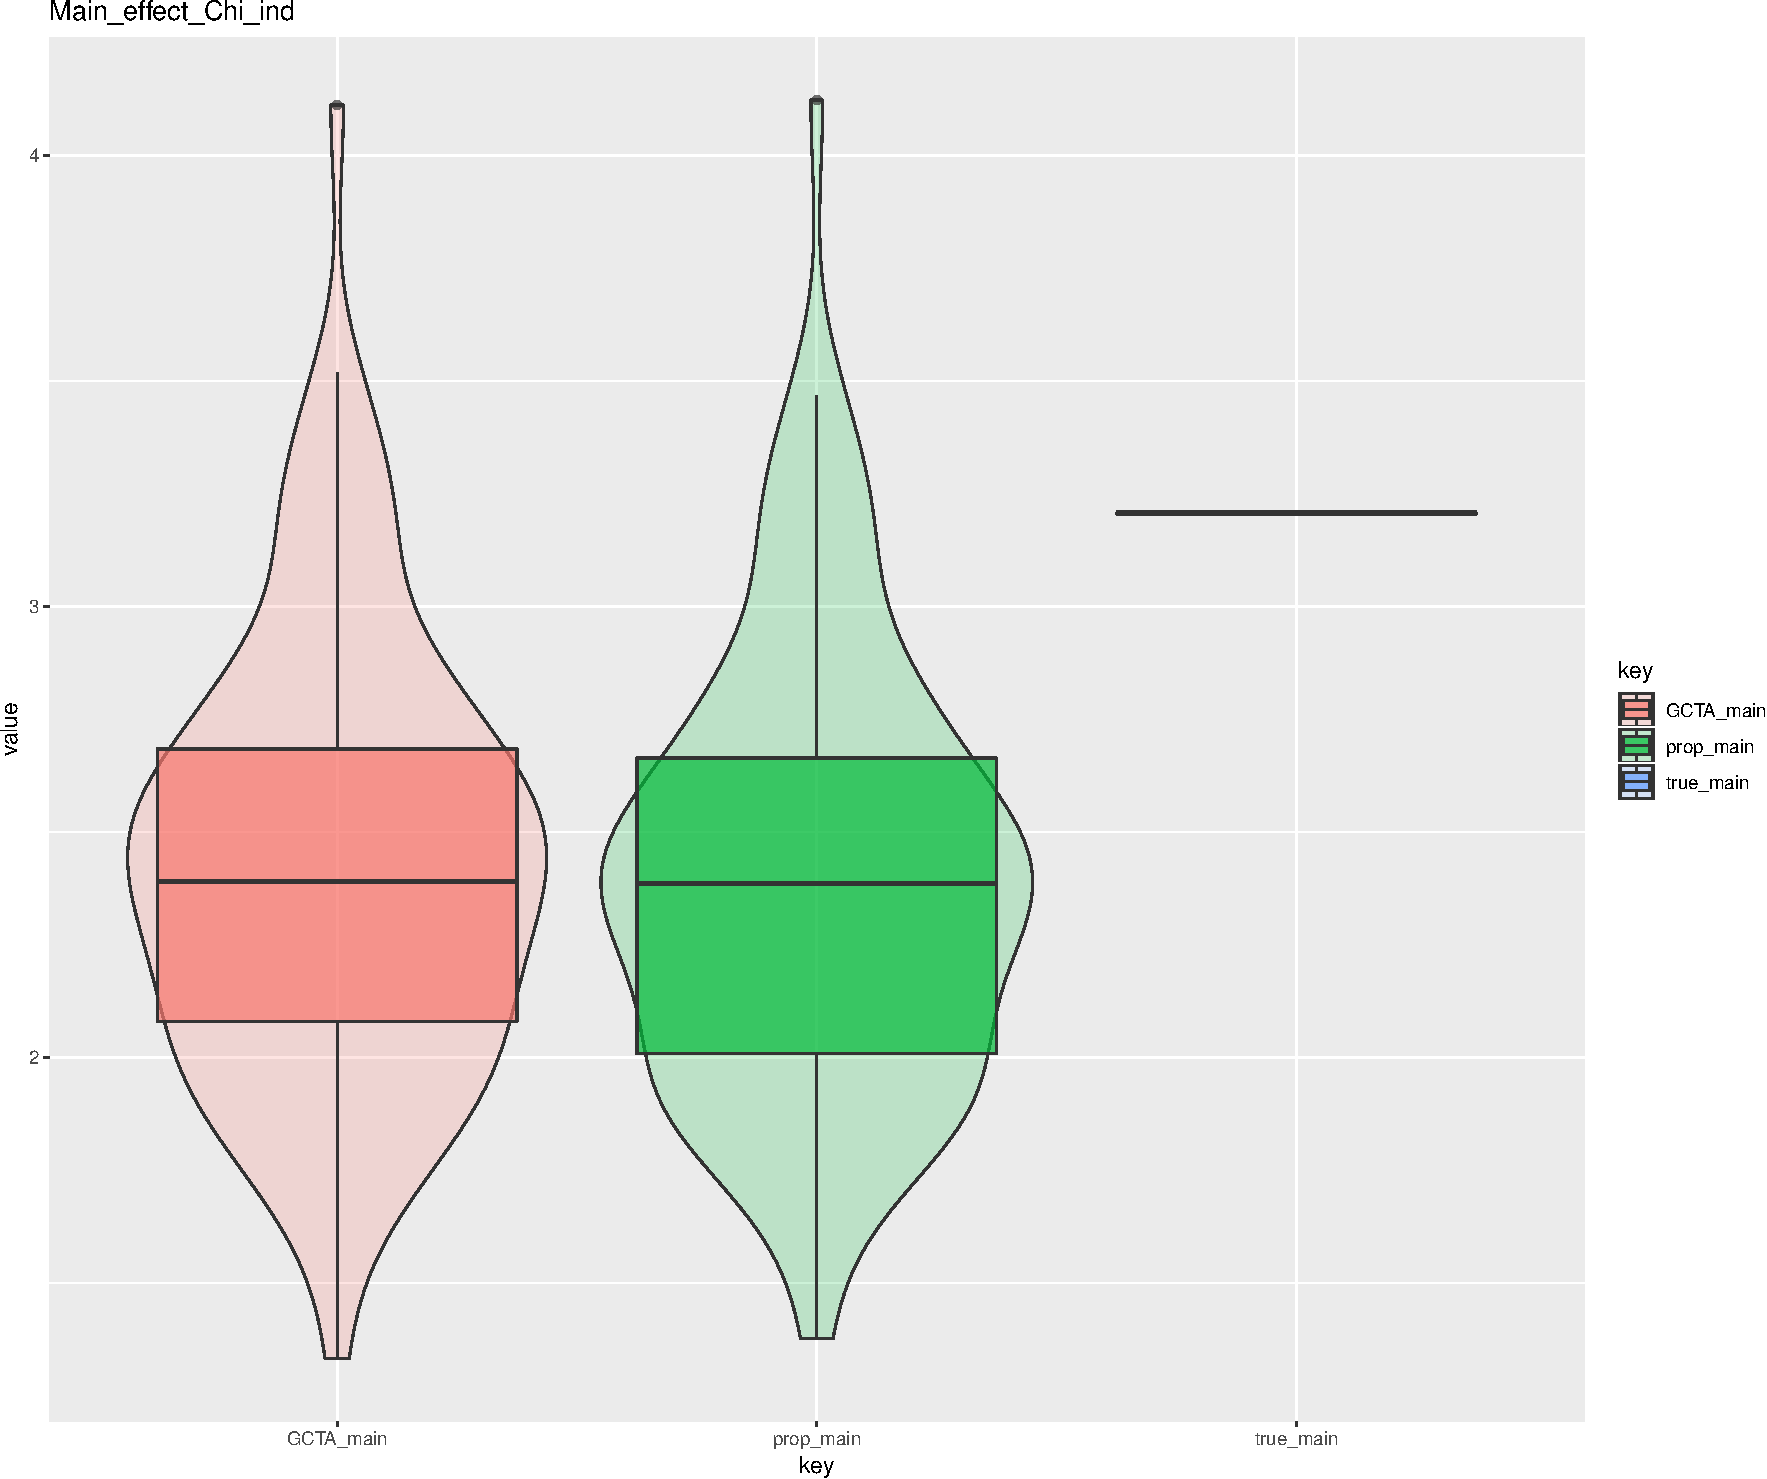
\includegraphics{Norl_cor_simulation_files/figure-latex/chi_main-1.pdf}

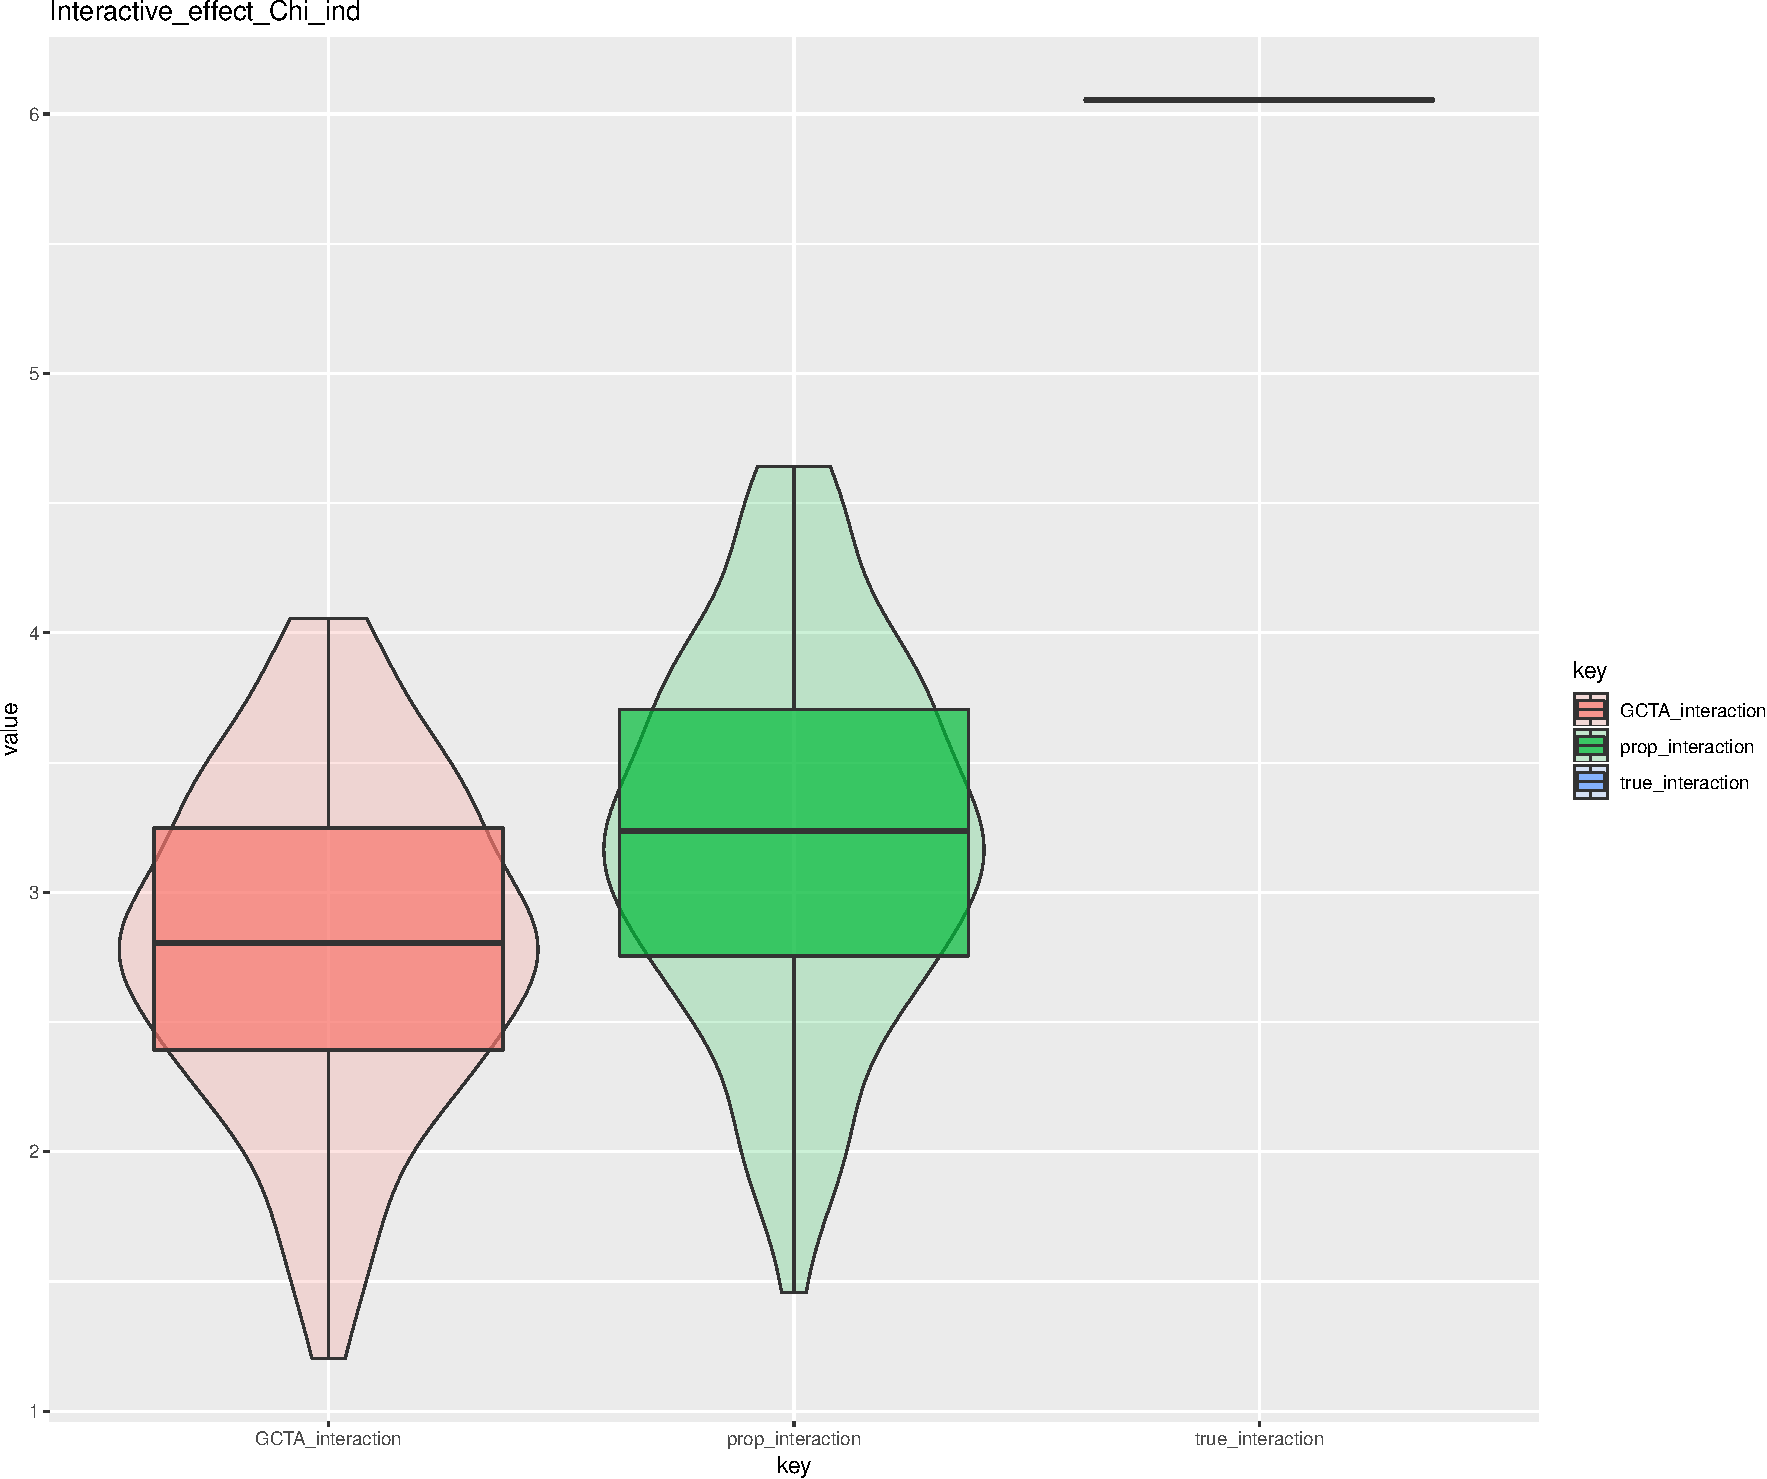
\includegraphics{Norl_cor_simulation_files/figure-latex/chi_inter-1.pdf}

\section{Conclusion}\label{conclusion}

\section{Further work}\label{further-work}


\end{document}
